\documentclass[fleqn, usenatbib, useAMS, a4paper]{mnras}
\usepackage{graphicx}
\usepackage{amsmath,paralist,xcolor,xspace,amssymb}
\usepackage{times}
\usepackage{comment}

\newcommand{\gadget}{{\sc Gadget}\xspace}
\newcommand{\swift}{{\sc Swift}\xspace}
\newcommand{\nbody}{$N$-body\xspace}

%opening
\title{FMM in SWIFT}
\author{Matthieu Schaller}
\begin{document}

\date{\today}

\pagerange{\pageref{firstpage}--\pageref{lastpage}} \pubyear{2014}

\maketitle

\label{firstpage}

\begin{abstract}
Making gravity great again.
\end{abstract}

\begin{keywords}
\end{keywords}

\section{Gravity in \swift}
\label{sec:gravity}

\subsection{Gravitational softening}
\label{ssec:potential_softening}

To avoid artificial two-body relaxation, the Dirac
$\delta$-distribution of particles is convolved with a softening
kernel of a given fixed, but time-variable, scale-length
$\epsilon$. Instead of the commonly used spline kernel of
\cite{Monaghan1985} (e.g. in \textsc{Gadget}), we use a C2 kernel
\citep{Wendland1995} which leads to an expression for the force that
is cheaper to compute and has a very similar overall shape. The C2
kernel has the advantage of being branch-free leading to an expression
which is faster to evaluate using vector units available on modern
architectures; it also does not require any divisions to evaluate the
softened forces. We set $\tilde\delta(\mathbf{x}) =
\rho(|\mathbf{x}|) = W(|\mathbf{x}|, 3\epsilon_{\rm Plummer})$, with
$W(r, H)$ given by

\begin{align}
W(r,H) &= \frac{21}{2\pi H^3} \times \nonumber \\
&\left\lbrace\begin{array}{rcl}
4u^5 - 15u^4 + 20u^3 - 10u^2 + 1 & \mbox{if} & u < 1,\\
0 & \mbox{if} & u \geq 1,
\end{array}
\right.
\end{align}
and $u = r/H$. The potential $\varphi(r,H)$ corresponding to this density distribution reads
\begin{align}
\varphi = 
\left\lbrace\begin{array}{rcl}
\frac{1}{H} (-3u^7 + 15u^6 - 28u^5 + 21u^4 - 7u^2 + 3) & \mbox{if} & u < 1,\\
\frac{1}{r} & \mbox{if} & u \geq 1.
\end{array}
\right.
\label{eq:fmm:potential}
\end{align}

These choices, lead to a potential at $|\mathbf{x}| = 0$ equal to the
central potential of a Plummer sphere (i.e. $1/\epsilon_{\rm
Plummer}$)\footnote{Note the factor $3$ in the definition of
$\rho(|\mathbf{x}|)$ which differs from the factor $2.8$ used
in \textsc{Gadget} as a consequence of the change of kernel
shape.}. The softened density profile, its corresponding potential and
resulting forces are shown on Fig. \ref{fig:fmm:softening} (for
details see Sec. 2 of~\cite{Price2007}).


\begin{figure}
\includegraphics[width=\columnwidth]{potential.pdf}
\caption{The density (top), potential (middle) and forces (bottom)
  generated py a point mass in our softened gravitational scheme.
  A Plummer-equivalent sphere is shown for comparison. The spline
  kernel of \citet{Monaghan1985}, used in \textsc{Gadget}, is shown
  for comparison but note that it has not been re-scaled to match the
  Plummer-sphere potential at $r=0$.  %(for completeness, we chose
  %$\epsilon=2$).
  }
\label{fig:fmm:softening}
\end{figure}

\subsection{Evaluating the forces using the Fast Multipole Method}
\label{ssec:fmm_summary}

The algorithmically challenging aspect of the \nbody problem is to
evaluate for each particle in a system the potential and associated
forces generated by all the other particles. Mathematically, this means
evaluate
\begin{equation}
  \phi(\mathbf{x}_a) = \sum_{b \neq a} G m_b\varphi(\mathbf{x}_a -
  \mathbf{x}_b)\qquad \forall~a\in N
  \label{eq:fmm:n_body}
\end{equation}
efficiently for large numbers of particles $N$. In the case of collisionless
dynamics, the particles are a mere Monte-Carlo sampling of the
underlying coarse-grained phase-space distribution which justifies the
use of approximate method to evaluate Eq.~\ref{eq:fmm:n_body}. The
\emph{Fast Multipole Method} (FMM) \citep{Greengard1987, Cheng1999},
popularized in the field and adapted specifically for gravity solvers
by \cite{Dehnen2000, Dehnen2002}, is an $\mathcal{O}(N)$ method
designed to solve Eq.~\ref{eq:fmm:n_body} by expanding the potential both
around $\mathbf{x}_i$ and $\mathbf{x}_j$ and grouping similar terms
arising from nearby particles. \\

In what follows, we use the compact multi-index notation of
\cite{Dehnen2014} (repeated in appendix \ref{sec:multi_index_notation}
for completeness) to simplify expressions and ease
comparisons. $\mathbf{k}$, $\mathbf{m}$ and $\mathbf{n}$ are
multi-indices and $\mathbf{r}$, $\mathbf{R}$, $\mathbf{x}$,
$\mathbf{y}$ and $\mathbf{z}$ are vectors, whilst $a$ and $b$ are
particle indices.\\

\begin{figure}
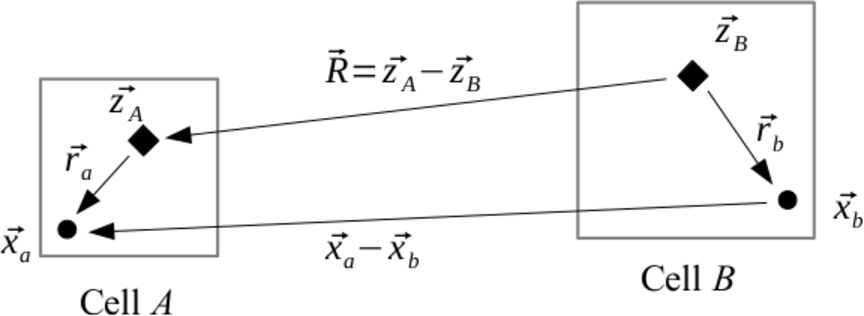
\includegraphics[width=\columnwidth]{cells.pdf}
\caption{The basics of the FMM: The potential generated by a particle
  at position $\mathbf{x}_b$ on a particle at position at location
  $\mathbf{x}_a$ is replaced by a Taylor expansion of the potential
  around the distance vector $\mathbf{R}$ linking the two centres of mass
  ($\mathbf{z}_A$ and $\mathbf{z}_B$) of cell $A$ and $B$. The
  expansion converges towards the exact expression provided
  $|\mathbf{R}|<|\mathbf{r}_a + \mathbf{r}_b|$.}
\label{fig:fmm:cells}
\end{figure}


For a single pair of particles $a$ and $b$ located in cell $A$ and $B$
with centres of mass $\mathbf{z}_A$ and  $\mathbf{z}_B$
respectively, as shown on Fig.~\ref{fig:fmm:cells}, the potential
generated by $b$ at the location of $a$ can be rewritten as
\begin{align}
  \varphi(\mathbf{x}_a - \mathbf{x}_b)
  &= \varphi\left(\mathbf{x}_a - \mathbf{z}_A - \mathbf{x}_b +
  \mathbf{z}_B + \mathbf{z}_A - \mathbf{z}_B\right)  \nonumber \\
  &= \varphi\left(\mathbf{r}_a - \mathbf{r}_b + \mathbf{R}\right)
  \nonumber \\
  &= \sum_\mathbf{k} \frac{1}{\mathbf{k}!} \left(\mathbf{r}_a -
  \mathbf{r}_b\right)^{\mathbf{k}} \nabla^{\mathbf{k}}\varphi(\mathbf{R})
  \nonumber \\
  &= \sum_\mathbf{k} \frac{1}{\mathbf{k}!} \sum_{\mathbf{n} <
    \mathbf{k}} \binom{\mathbf{k}}{\mathbf{n}} \mathbf{r}_a^{\mathbf{n}}
  \left(-\mathbf{r}_b\right)^{\mathbf{k} - \mathbf{n}}
  \nabla^{\mathbf{k}}\varphi(\mathbf{R})\nonumber \\
  &= \sum_\mathbf{n} \frac{1}{\mathbf{n}!} \mathbf{r}_a^{\mathbf{n}}
  \sum_\mathbf{m} \frac{1}{\mathbf{m}!}
  \left(-\mathbf{r}_b\right)^\mathbf{m} \nabla^{\mathbf{n}+\mathbf{m}} \varphi(\mathbf{R}),
\end{align}
where we used the Taylor expansion of $\varphi$ around $\mathbf{R} \equiv
\mathbf{z}_A - \mathbf{z}_B$ on the third line, used $\mathbf{r}_a
\equiv \mathbf{x}_a - \mathbf{z}_A$, $\mathbf{r}_b \equiv \mathbf{x}_b
- \mathbf{z}_B$ throughout and defined $\mathbf{m} \equiv
\mathbf{k}-\mathbf{n}$ on the last line. Expanding the series only up
to order $p$, we get
\begin{equation}
  \varphi(\mathbf{x}_a - \mathbf{x}_b) \approx \sum_{\mathbf{n}}^{p}
  \frac{1}{\mathbf{n}!} \mathbf{r}_a^{\mathbf{n}} \sum_{\mathbf{m}}^{p
    -|\mathbf{n}|} 
  \frac{1}{\mathbf{m}!} \left(-\mathbf{r}_b\right)^\mathbf{m}
  \nabla^{\mathbf{n}+\mathbf{m}} \varphi(\mathbf{R}),
  \label{eq:fmm:fmm_one_part}
\end{equation}
with the approximation converging as $p\rightarrow\infty$ towards the
correct value provided $|\mathbf{R}|<|\mathbf{r}_a +
\mathbf{r}_b|$. If we now consider all the particles within $B$ and
combine their contributions to the potential at location
$\mathbf{x}_a$ in cell $A$, we get
\begin{align}
  \phi_{BA}(\mathbf{x}_a) &= \sum_{b\in B}G m_b\varphi(\mathbf{x}_a -
  \mathbf{x}_b)  \label{eq:fmm:fmm_one_cell}  \\
  &\approx G\sum_{\mathbf{n}}^{p}
  \frac{1}{\mathbf{n}!} \mathbf{r}_a^{\mathbf{n}} \sum_{\mathbf{m}}
    ^{p -|\mathbf{n}|}
  \frac{1}{\mathbf{m}!} \sum_{b\in B} m_b\left(-\mathbf{r}_b\right)^\mathbf{m}
  \nabla^{\mathbf{n}+\mathbf{m}} \varphi(\mathbf{R}) \nonumber. 
\end{align}
This last equation forms the basis of the FMM. The algorithm
decomposes the equation into three separated sums evaluated at
different stages.\\

In a first step, multipoles are constructed from the
innermost sum. For each cell, we compute all the terms
\begin{equation}
  \mathsf{M}_{\mathbf{m}}(\mathbf{z}_B) = \frac{1}{\mathbf{m}!}
  \sum_{b\in B} m_b\left(-\mathbf{r}_b\right)^\mathbf{m} \label{eq:fmm:P2M} 
\end{equation}
up to order $p$. This is the first kernel of the method, commonly
labelled as \textsc{P2M} (particle to multipole). In a second step, we
compute the second kernel, \textsc{M2L} (multipole to local
expansion), which corresponds to the interaction of a cell with
another one:
\begin{equation}
  \mathsf{F}_{\mathbf{n}}(\mathbf{z}_A) = G\sum_{\mathbf{m}}^{p -|\mathbf{n}|}
  \mathsf{M}_{\mathbf{m}}(\mathbf{z}_B)
  \mathsf{D}_{\mathbf{n}+\mathbf{m}}(\mathbf{R}), \label{eq:fmm:M2L} 
\end{equation}
where $\mathsf{D}_{\mathbf{n}+\mathbf{m}}(\mathbf{R}) \equiv
\nabla^{\mathbf{n}+\mathbf{m}} \varphi(\mathbf{R})$ is an order $n+m$
derivative of the potential. This is the computationally expensive
step of the FMM algorithm as the number of operations in a naive
implementation using cartesian coordinates scales as
$\mathcal{O}(p^6)$. More advanced techniques
\citep[e.g.][]{Dehnen2014} can bring the cost down to
$\mathcal{O}(p^3)$, albeit at a considerable algebraic cost. For
collisionless dynamics, high accuracy is not required and low values
of $p$ are sufficient, which maintains the computational cost of the
M2L kernel at a reasonable level.  
Finally, in the last step, the potential is propagated from the local
expansion centre to the particles (L2P kernel) using
\begin{equation}
  \phi_{BA}(\mathbf{x}_a) = \sum_{\mathbf{n}}^{p}
  \frac{1}{\mathbf{n}!} \mathbf{r}_a^{\mathbf{n}}
  \mathsf{F}_{\mathbf{n}}(\mathbf{z}_A). \label{eq:fmm:L2P} 
\end{equation}
In summary, the potential generated by a cell $B$ on the particles in
cell $A$ is obtained by the successive application of the P2M, M2L and
L2P kernels. The P2M and L2P kernels are applied only once per
particle, whilst one M2L calculation has to be performed for each pair
of cells. The forces applied to the particles are obtained by the same
procedure using an extra order in the Taylor expansion. For instance,
for the acceleration along $x$, we have:
\begin{equation}
  a_x(\mathbf{x}_a) = \sum_{\mathbf{n}}^{p-1}
  \frac{1}{\mathbf{n}!} \mathbf{r}_a^{\mathbf{n}}
  \mathsf{F}_{\mathbf{n}+\left(1,0,0\right)}(\mathbf{z}_A). \label{eq:fmm:L2P_force} 
\end{equation}

In practice, the multipoles can be constructed recursively from the
leaves of the tree to the root and the local expansions from the root
to the leaves by shifting the $\mathsf{M}$ and $\mathsf{F}$ tensors
and adding their contributions to their parent or daughter cell's
tensors respecitvely. The shifting formulas (M2M and L2L kernels)
read:

\begin{align}
  \mathsf{M}_{\mathbf{m}}(\mathbf{x} + \mathbf{y}) &=
  \sum_{\mathbf{n}}^{\mathbf{m}}
  \frac{\mathbf{y}^\mathbf{n}}{\mathbf{n}!}\mathsf{M}_{\mathbf{m} -
    \mathbf{n}}(\mathbf{x}), \label{eq:fmm:M2M} \\
  \mathsf{F}_{\mathbf{n}}(\mathbf{x} + \mathbf{y}) &=
  \sum_{\mathbf{m}}^{p-|\mathbf{n}|}
  \frac{\mathbf{y}^\mathbf{m}}{\mathbf{m}!}\mathsf{F}_{\mathbf{m} +
    \mathbf{n}}(\mathbf{x}). \label{eq:fmm:L2L} 
\end{align}

All the kernels (Eqs.~\ref{eq:fmm:P2M}-\ref{eq:fmm:L2L}) are rather
straightforward to evaluate as they are only made of additions and
multiplications (provided $\mathsf{D}$ can be evaluated quickly, see
Sec.~\ref{ssec:grav_derivatives}), which are extremely efficient
instructions on modern architectures. However, the fully expanded sums
can lead to rather large and prone to typo expressions. To avoid any
mishaps, we use a \texttt{python} script to generate C code in which
all the sums are unrolled and correct by construction. In \swift, we
implemented the kernels up to order $p=5$, as it proved to be accurate
enough for our purpose, but this could be extended to higher order
easily. This implies storing $56$ numbers per cell for each
$\textsf{M}$ and $\textsf{F}$ plus three numbers for the location of
the centre of mass. For leaf-cells with large numbers of particles, as
in \swift, this is a small memory overhead. One further small
improvement consists in choosing $\mathbf{z}_A$ to be the centre of
mass of cell $A$ rather than its geometrical centre. The first order
multipoles ($\mathsf{M}_{100},\mathsf{M}_{010},\mathsf{M}_{001}$) then
vanish by construction. This allows us to simplify some of the
expressions and helps reduce, albeit by a small fraction, the memory
footprint of the tree structure.

%\subsection{Notes on the derivatives of the gravitational potential}
\label{ssec:grav_derivatives}

The calculation of all the
$\mathsf{D}_\mathbf{n}(x,y,z) \equiv \nabla^{\mathbf{n}}\varphi(x,y,z)$ terms up
to the relevent order can be quite tedious and it is beneficial to
automatize the whole setup. Ideally, one would like to have an
expression for each of these terms that is only made of multiplications
and additions of each of the coordinates and the inverse distance. We
achieve this by writing $\varphi$ as a composition of functions
$\varphi(u(x,y,z))$ and apply the \textit{Fa\`a di Bruno}
formula \citep[i.e. the ``chain rule'' for higher order derivatives,
 see e.g.][]{Hardy2006} to construct our terms:
\begin{equation}
\label{eq:faa_di_bruno}
\frac{\partial^n}{\partial x_1 \cdots \partial x_n} \varphi(u)
= \sum_{A} \varphi^{(|A|)}(u) \prod_{B \in
A} \frac{\partial^{|B|}}{\prod_{c\in B}\partial x_c} u(x,y,z),
\end{equation}
where $A$ is the set of all partitions of $\lbrace1,\cdots, n\rbrace$,
$B$ is a block of a partition in the set $A$ and $|\cdot|$ denotes the
cardinality of a set. For generic functions $\varphi$ and $u$ this
formula yields an untracktable number of terms; an 8th-order
derivative will have $4140$ (!)  terms in the sum\footnote{The number
  of terms in the sum is given by the Bell number of the same
  order.}. \\ For the un-softened gravitational potential, we choose to write
\begin{align}
   \varphi(x,y,z) &= 1 / \sqrt{u(x,y,z)}, \\
   u(x,y,z) &= x^2 + y^2 + z^2.
\end{align}
This choice allows to have derivatives of any order of $\varphi(u)$ that
can be easily expressed and only depend on powers of $u$:
\begin{equation}
\varphi^{(n)}(u) = (-1)^n\cdot\frac{(2n-1)!!}{2^n}\cdot\frac{1}{u^{n+\frac{1}{2}}},
\end{equation}
where $!!$ denotes the semi-factorial. More importantly, this
choice of decomposition allows us to have non-zero derivatives of $u$
only up to second order in $x$, $y$ or $z$. The number of non-zero
terms in eq. \ref{eq:faa_di_bruno} is hence drastically reduced. For
instance, when computing $\mathsf{D}_{(4,1,3)}(\mathbf{r}) \equiv
\frac{\partial^8}{\partial x^4 \partial y \partial z^3}
\varphi(u(x,y,z))$, $4100$ of the $4140$ terms will involve at least one
zero-valued derivative (e.g. $\partial^3/\partial x^3$ or
$\partial^2/\partial x\partial y$) of $u$. Furthermore, among the 40
remaining terms, many will involve the same combination of derivatives
of $u$ and can be grouped together, leaving us with a sum of six
products of $x$,$y$ and $z$. This is generally the case for most of
the $\mathsf{D}_\mathbf{n}$'s and figuring out which terms are identical in a
given set of partitions of $\lbrace1,\cdots, n\rbrace$ is an
interesting exercise in combinatorics left for the reader \citep[see
  also][]{Hardy2006}. We use a \texttt{python} script based on this
technique to generate the actual C routines used within \swift. Some
examples of these terms are given in Appendix
\ref{sec:pot_derivatives}.


\subsection{Coupling the FMM to a mesh for periodic long-range forces}
\label{ssec:mesh_summary}

We truncate the potential and forces computed via the FMM using a
smooth function that drops quickly to zero at some scale $r_s$ set by
the top-level mesh. Traditionally, implementations have used
expressions which are cheap to evaluate in Fourier space
\citep[e.g.][]{Bagla2003, Springel2005}. This, however, implies a
large cost for each interaction computed within the tree as the
real-space truncation function won't have a simple analytic form that
can be evaluated efficiently even by modern architectures (typically
an $\mathrm{erf}()$ function). Since the FMM scheme involves to not
only evaluate the forces but higher-order derivatives, a more
appropiate choice is necessary. We use the sigmoid
$\sigma(w) \equiv \frac{e^w}{1 + e^w}$ as the basis of our truncation
function and write for the potential:

\begin{align}
  \varphi_s(r) &= \frac{1}{r} \times \chi(r, r_s) = \frac{1}{r}\times\left[2 - 2\sigma\left(\frac{2r}{r_s}\right)\right].% \nonumber\\
  %&= \frac{1}{r}\left[2 - \frac{2e^{\frac{2r}{r_s}}}{1+e^{\frac{2r}{r_s}}}.\right] 
\end{align}
This function alongside the trunctation function used in
\gadget\footnote{For completeness, the \gadget expression reads:\\
 $\varphi_s(r) = \frac{1}{r} \times \mathrm{erfc}(\frac{1}{2}\frac{r}{r_s})$.} is shown
on Fig.~\ref{fig:fmm:potential_short}. This choice of $\sigma(w)$ can
seem rather cumbersome at first but writing
$\alpha(w) \equiv (1+e^w)^{-1}$, one can express all derivatives of
$\sigma(w)$ as simple polynomials in $\alpha(w)$ (with an identical
$e^w$ pre-factor), which are easy and cheap to evaluate (see Appendix
\ref{sec:pot_derivatives}). For instance, in the case of the direct
force evaluation between two particles, we obtain
\begin{align}
  |\mathbf{f}_s(r)| &= \left|\frac{\partial}{\partial r}\varphi_s(r)\right|
                      = \left|\frac{\partial}{\partial r}\left(\frac{1}{r} \chi(r, r_s)\right) \right|\nonumber \\
  &=  \frac{1}{r^2}\times\left[-\frac{4r}{r_s}\sigma'\left(\frac{2r}{r_s}\right) -
    2\sigma\left(\frac{2r}{r_s}\right) + 2\right] \nonumber \\
  &=
  % \frac{1}{r^2}\times 2 \left[x\alpha(x) - x\alpha(x)^2 - e^x\alpha(x) + 1\right],
  % \frac{1}{r^2}\times 2 \left[1 - e^x\alpha(x) - xe^x\alpha^2(x)\right],
    \frac{1}{r^2}\times 2 \left[1 - e^x\left(\alpha(x) - x\alpha(x)^2\right) \right]
\end{align}
with $x\equiv2r/r_s$. The truncated force is compared to the Newtonian
force and to the \gadget truncated forces\footnote{For completeness,
  the \gadget expression for the norm of the truncated forces is:
  $|\mathbf{f}_s(r)| = \frac{1}{r^2} \times
  \left[\mathrm{erfc}\left(\frac{1}{2}\frac{r}{r_s}\right) +
    \frac{1}{\sqrt{\upi}}\frac{r}{r_s}\exp\left(-\frac{1}{4}\frac{r^2}{r_s^2}\right)\right]$.}
on Fig.~\ref{fig:fmm:force_short}. At distance $r<r_s/10$, the
truncation term is negligibly close to one and the truncated forces
can be replaced by their Newtonian equivalent. We use this
optimization in \swift and only compute truncated forces between pairs
of particles that are in tree-leaves larger than $1/10$ of the mesh
size or between
two tree-leaves distant by more than that amount.\\

\textcolor{red}{MORE WORDS HERE.}\\

The truncation function in Fourier space reads

\begin{equation}
  \tilde\varphi_l(k) =
  \frac{1}{k^2}\left[\frac{\upi}{2}kr_s\textrm{csch}\left(\frac{\upi}{2}kr_s\right)
    \right]
\end{equation}

\begin{figure}
\includegraphics[width=\columnwidth]{potential_short.pdf}
\caption{Truncated potential used in \swift (green line) and \gadget
  (yellow line) alongside the full Newtonian potential (blue dasheed
  line). The green dash-dotted line corresponds to the same
  trunctation function where the exponential in the sigmoid is
  replaced by a sixth order Taylor expansion. At $r>4r_s$, the
  truncated potential becomes negligible.}
\label{fig:fmm:potential_short}
\end{figure}



\begin{figure}
\includegraphics[width=\columnwidth]{force_short.pdf}
\caption{Norm of the truncated forces used in \swift (green line) and
  \gadget (yellow line) alongside the full Newtonian force term (blue
  dasheed line). The green dash-dotted line corresponds to the same
  trunctation function where the exponential in the sigmoid is
  replaced by a sixth order Taylor expansion. At $r<r_s/10$, the
  truncated forces becomes almost equal to the Newtonian ones and can
  safely be replaced by their simpler form. The deviation between the
  exact expression and the one obtained from Taylor expansion at
  $r>r_s$ has a small impact since no pairs of particles should
  interact directly over distances of order the mesh size. }
\label{fig:fmm:force_short}
\end{figure}


\begin{figure}
\includegraphics[width=\columnwidth]{potential_long.pdf}
\caption{cc}
\label{fig:fmm:potential_long}
\end{figure}


\subsubsection{Normalisation of the potential}

The gravitational potential computed by the combination of the mesh
and multipole method needs to be corrected to obtain the zero point of
the peculiar potential. Learning from the Ewald summation technique
(see Sec.~\ref{ssec:exact_forces}), we notice that of the three terms
entering the calculation of the potential with periodic boundary
conditions (see Eq. 2.11 of \cite{Hernquist1991}), the last two are
computed by the mesh and tree respectively. The only reamining term is
the constant
\begin{equation}
  \frac{4\pi r_s^2}{L^3}\sum_a m_a,
\end{equation}
where the sum runs over all particles and $L$ is the comoving
side-length of the simulation volume. This constant is added to the
potential of all the particles in the simulation.


\bibliographystyle{mnras}
\bibliography{./bibliography.bib}

\appendix
\input{vector_notation}
\onecolumn
\section{Derivatives of the potential}
\label{sec:pot_derivatives}

For completeness, we give here the full expression for the first few
derivatives of the potential that are used in our FMM scheme. We use
the notation $\mathbf{r}=(r_x, r_y, r_z)$, $r = |\mathbf{r}|$ and
$u=r/H$. We can construct the higher order derivatives by successively
applying the "chain rule". We show representative examples of the
first few relevant ones here split by order. We start by constructing
common quantities that appear in derivatives of multiple orders.

\begin{align}
  \mathsf{\tilde{D}}_{1}(r, u, H) =
  \left\lbrace\begin{array}{rcl}
  \left(-3u^7 + 15u^6 - 28u^5 + 21u^4 - 7u^2 + 3\right)\times  H^{-1} & \mbox{if} & u < 1,\\
  r^{-1} & \mbox{if} & u \geq 1, 
  \end{array}
  \right.\nonumber
\end{align}
%%%%%%%%%%%%%%%%%%%%%%%%%%%%%%%%%%
\begin{align}
  \mathsf{\tilde{D}}_{3}(r, u, H) =
  \left\lbrace\begin{array}{rcl}
  -\left(21u^5 - 90u^4 + 140u^3 -84u^2 +14\right)\times  H^{-3}& \mbox{if} & u < 1,\\
  -1 \times r^{-3} & \mbox{if} & u \geq 1, 
  \end{array}
  \right.\nonumber
\end{align}
%%%%%%%%%%%%%%%%%%%%%%%%%%%%%%%%%%
\begin{align}
  \mathsf{\tilde{D}}_{5}(r, u, H) =
  \left\lbrace\begin{array}{rcl}
  \left(-105u^3 + 360u^2 - 420u + 168\right)\times  H^{-5}& \mbox{if} & u < 1,\\
  3\times r^{-5} & \mbox{if} & u \geq 1, 
  \end{array}
  \right.\nonumber
\end{align}
%%%%%%%%%%%%%%%%%%%%%%%%%%%%%%%%%%
\begin{align}
  \mathsf{\tilde{D}}_{7}(r, u, H) =
  \left\lbrace\begin{array}{rcl}
  -\left(315u - 720 + 420u^{-1}\right)\times  H^{-7} & \mbox{if} & u < 1,\\
  -15\times r^{-7} & \mbox{if} & u \geq 1, 
  \end{array}
  \right.\nonumber
\end{align}
%%%%%%%%%%%%%%%%%%%%%%%%%%%%%%%%%%
\begin{align}
  \mathsf{\tilde{D}}_{9}(r, u, H) =
  \left\lbrace\begin{array}{rcl}
  \left(-315u^{-1} + 420u^{-3}\right)\times  H^{-9}& \mbox{if} & u < 1,\\
  105\times r^{-9} & \mbox{if} & u \geq 1.
  \end{array}
  \right.\nonumber
\end{align}
Starting from the potential (Eq. \ref{eq:fmm:potential},
reproduced here for completeness), we can now build all the relevent derivatives
\begin{align}
  \mathsf{D}_{000}(\mathbf{r}) = \varphi (\mathbf{r},H) =
    \mathsf{\tilde{D}}_{1}(r, u, H) \nonumber
\end{align}

\noindent\rule{6cm}{0.4pt}
\begin{align}
  \mathsf{D}_{100}(\mathbf{r}) = \frac{\partial}{\partial r_x} \varphi (\mathbf{r},H) =
    r_x \mathsf{\tilde{D}}_{3}(r, u, H) \nonumber
\end{align}

\noindent\rule{6cm}{0.4pt}
\begin{align}
\mathsf{D}_{200}(\mathbf{r}) = \frac{\partial^2}{\partial r_x^2} \varphi (\mathbf{r},H) = 
r_x^2 \mathsf{\tilde{D}}_{5}(r, u, H) +
\mathsf{\tilde{D}}_{3}(r, u, H)\nonumber
\end{align}

\begin{align}
\mathsf{D}_{110}(\mathbf{r}) = \frac{\partial^2}{\partial r_x\partial r_y} \varphi (\mathbf{r},H) = 
   r_x r_y \mathsf{\tilde{D}}_{5}(r, u, H) \nonumber
\end{align}

\noindent\rule{6cm}{0.4pt}
\begin{align}
\mathsf{D}_{300}(\mathbf{r}) = \frac{\partial^3}{\partial r_x^3} \varphi (\mathbf{r},H) = 
  r_x^3 \mathsf{\tilde{D}}_{7}(r, u, H)
  + 3 r_x \mathsf{\tilde{D}}_{5}(r, u, H) \nonumber
\end{align}

\begin{align}
\mathsf{D}_{210}(\mathbf{r}) = \frac{\partial^3}{\partial r_x^2 r_y} \varphi (\mathbf{r},H) = 
r_x^2 r_y \mathsf{\tilde{D}}_{7}(r, u, H) +
r_y \mathsf{\tilde{D}}_{5}(r, u, H) \nonumber
\end{align}

\begin{align}
\mathsf{D}_{111}(\mathbf{r}) = \frac{\partial^3}{\partial r_x\partial r_y\partial r_z} \varphi (\mathbf{r},H) = 
  r_x r_y r_z \mathsf{\tilde{D}}_{7}(r, u, H) \nonumber
\end{align}

\noindent\rule{6cm}{0.4pt}
\begin{align}
  \mathsf{D}_{400}(\mathbf{r}) &= \frac{\partial^4}{\partial r_x^4}
  \varphi (\mathbf{r},H) =
  r_x^4 \mathsf{\tilde{D}}_{9}(r, u, H)+
  6r_x^2 \mathsf{\tilde{D}}_{7}(r, u, H) +
  3 \mathsf{\tilde{D}}_{5}(r, u, H)
  \nonumber
\end{align}

\begin{align}
  \mathsf{D}_{310}(\mathbf{r}) &= \frac{\partial^4}{\partial r_x^3
    \partial r_y} \varphi (\mathbf{r},H) =
  r_x^3 r_y \mathsf{\tilde{D}}_{9}(r, u, H) +
  3 r_x r_y \mathsf{\tilde{D}}_{7}(r, u, H)
  \nonumber
\end{align}

\begin{align}
  \mathsf{D}_{220}(\mathbf{r}) &= \frac{\partial^4}{\partial r_x^2
    \partial r_y^2} \varphi (\mathbf{r},H) =
    r_x^2 r_y^2 \mathsf{\tilde{D}}_{9}(r, u, H) +
    r_x^2 \mathsf{\tilde{D}}_{7}(r, u, H) +
    r_y^2 \mathsf{\tilde{D}}_{7}(r, u, H) +
    \mathsf{\tilde{D}}_{5}(r, u, H)
  \nonumber
\end{align}

\begin{align}
  \mathsf{D}_{211}(\mathbf{r}) &= \frac{\partial^4}{\partial r_x^2
    \partial r_y   \partial r_z} \varphi (\mathbf{r},H) =
    r_x^2 r_y r_z \mathsf{\tilde{D}}_{9}(r, u, H) +
    r_y r_z \mathsf{\tilde{D}}_{7}(r, u, H)
  \nonumber
\end{align}



\begin{comment}

\noindent\rule{6cm}{0.4pt}

\begin{align}
\mathsf{D}_{100}(\mathbf{r}) = \frac{\partial}{\partial r_x} \varphi (\mathbf{r},H) = 
\left\lbrace\begin{array}{rcl}
-\frac{r_x}{H^3} \left(21u^5 - 90u^4 + 140u^3 - 84u^2 + 14\right) & \mbox{if} & u < 1,\\
-\frac{r_x}{r^3} & \mbox{if} & u \geq 1, 
\end{array}
\right.\nonumber
\end{align}

\noindent\rule{6cm}{0.4pt}

\begin{align}
\mathsf{D}_{200}(\mathbf{r}) = \frac{\partial^2}{\partial r_x^2} \varphi (\mathbf{r},H) = 
\left\lbrace\begin{array}{rcl}
\frac{r_x^2}{H^5}\left(-105u^3+360u^2-420u+168\right) -
\frac{1}{H^3} \left(21u^5 - 90u^4 + 140u^3 - 84u^2 + 14\right) & \mbox{if} & u < 1,\\
3\frac{r_x^2}{r^5} - \frac{1}{r^3} & \mbox{if} & u \geq 1, 
\end{array}
\right.\nonumber
\end{align}

\begin{align}
\mathsf{D}_{110}(\mathbf{r}) = \frac{\partial^2}{\partial r_x\partial r_y} \varphi (\mathbf{r},H) = 
\left\lbrace\begin{array}{rcl}
\frac{r_xr_y}{H^5}\left(-105u^3+360u^2-420u+168\right) & \mbox{if} & u < 1,\\
3\frac{r_xr_y}{r^5} & \mbox{if} & u \geq 1, 
\end{array}
\right.\nonumber
\end{align}

\noindent\rule{6cm}{0.4pt}

\begin{align}
\mathsf{D}_{300}(\mathbf{r}) = \frac{\partial^3}{\partial r_x^3} \varphi (\mathbf{r},H) = 
\left\lbrace\begin{array}{rcl}
-\frac{r_x^3}{H^7} \left(315u - 720 + 420u^{-1}\right) +
\frac{3r_x}{H^5}\left(-105u^3+360u^2-420u+168\right) & \mbox{if} & u < 1,\\
-15\frac{r_x^3}{r^7} + 9 \frac{r_x}{r^5} & \mbox{if} & u \geq 1, 
\end{array}
\right.\nonumber
\end{align}

\begin{align}
\mathsf{D}_{210}(\mathbf{r}) = \frac{\partial^3}{\partial r_x^3} \varphi (\mathbf{r},H) = 
\left\lbrace\begin{array}{rcl}
-\frac{r_x^2r_y}{H^7} \left(315u - 720 + 420u^{-1}\right) +
\frac{r_y}{H^5}\left(-105u^3+360u^2-420u+168\right) & \mbox{if} & u < 1,\\
-15\frac{r_x^2r_y}{r^7} + 3 \frac{r_y}{r^5} & \mbox{if} & u \geq 1, 
\end{array}
\right.\nonumber
\end{align}


\begin{align}
\mathsf{D}_{111}(\mathbf{r}) = \frac{\partial^3}{\partial r_x\partial r_y\partial r_z} \varphi (\mathbf{r},H) = 
\left\lbrace\begin{array}{rcl}
-\frac{r_xr_yr_z}{H^7} \left(315u - 720 + 420u^{-1}\right) & \mbox{if} & u < 1,\\
-15\frac{r_xr_yr_z}{r^7} & \mbox{if} & u \geq 1, 
\end{array}
\right.\nonumber
\end{align}

\noindent\rule{6cm}{0.4pt}

\begin{align}
  \mathsf{D}_{400}(\mathbf{r}) &=
  \nonumber
\end{align}

\begin{align}
  \mathsf{D}_{310}(\mathbf{r}) &=
  \nonumber
\end{align}

\begin{align}
  \mathsf{D}_{220}(\mathbf{r}) &=
  \nonumber
\end{align}

\begin{align}
  \mathsf{D}_{211}(\mathbf{r}) &=
  \nonumber
\end{align}

\end{comment}



\label{lastpage}

\end{document}
